\section{Методика изготовления нанодимеров}

На данный момент существует достаточно много способов изготовления планарных наноструктур различных размеров и форм, и наиболее распространенными являются различные виды литографии \cite{nanotechnologybook}. В этом методе изображение элемента или схемы выполняется в виде рисунка на металлической пленке, нанесенной на прозрачную подложку. Такой рисунок называется маской или шаблоном. Затем рисунок с помощью потока электронов переносится на полупроводниковую пластину, в которой слой за слоем формируется физическая структура требуемого объекта. Таким образом, литография -- процесс переноса изображения с маски на подложку. Для этого на поверхности подложки создается пленочное покрытие из полимерного материала -- резиста; покрытие облучают через маску с изображением элементов схемы и затем покрытие проявляют (травят в растворителе) так, что изображение схемы переносится на подложку.

Существует два основных вида резистов: позитивные и негативные. Если в результате облучения резист полимеризуется и теряет растворимость, то обработка растворителем (проявление) ведет к удалению только необлученных участков и на подложке возникает негативное изображение маски. Соответствующие резисты называются негативными. Если же в результате воздействия облучения резист становится растворимым, то при облучении через маску и последующим проявлении удаляются облученные участки и на подложке возникает позитивное изображение маски. Такие резисты называются позитивными. На рис.~\ref{img:litography} слева приведен процесс проявления образца с пленкой негативного резиста, а справа -- позитивного. Далее такая структура подвергается травлению, и в результате получается массив объектов на поверхности подложки.

\begin{figure}
\center{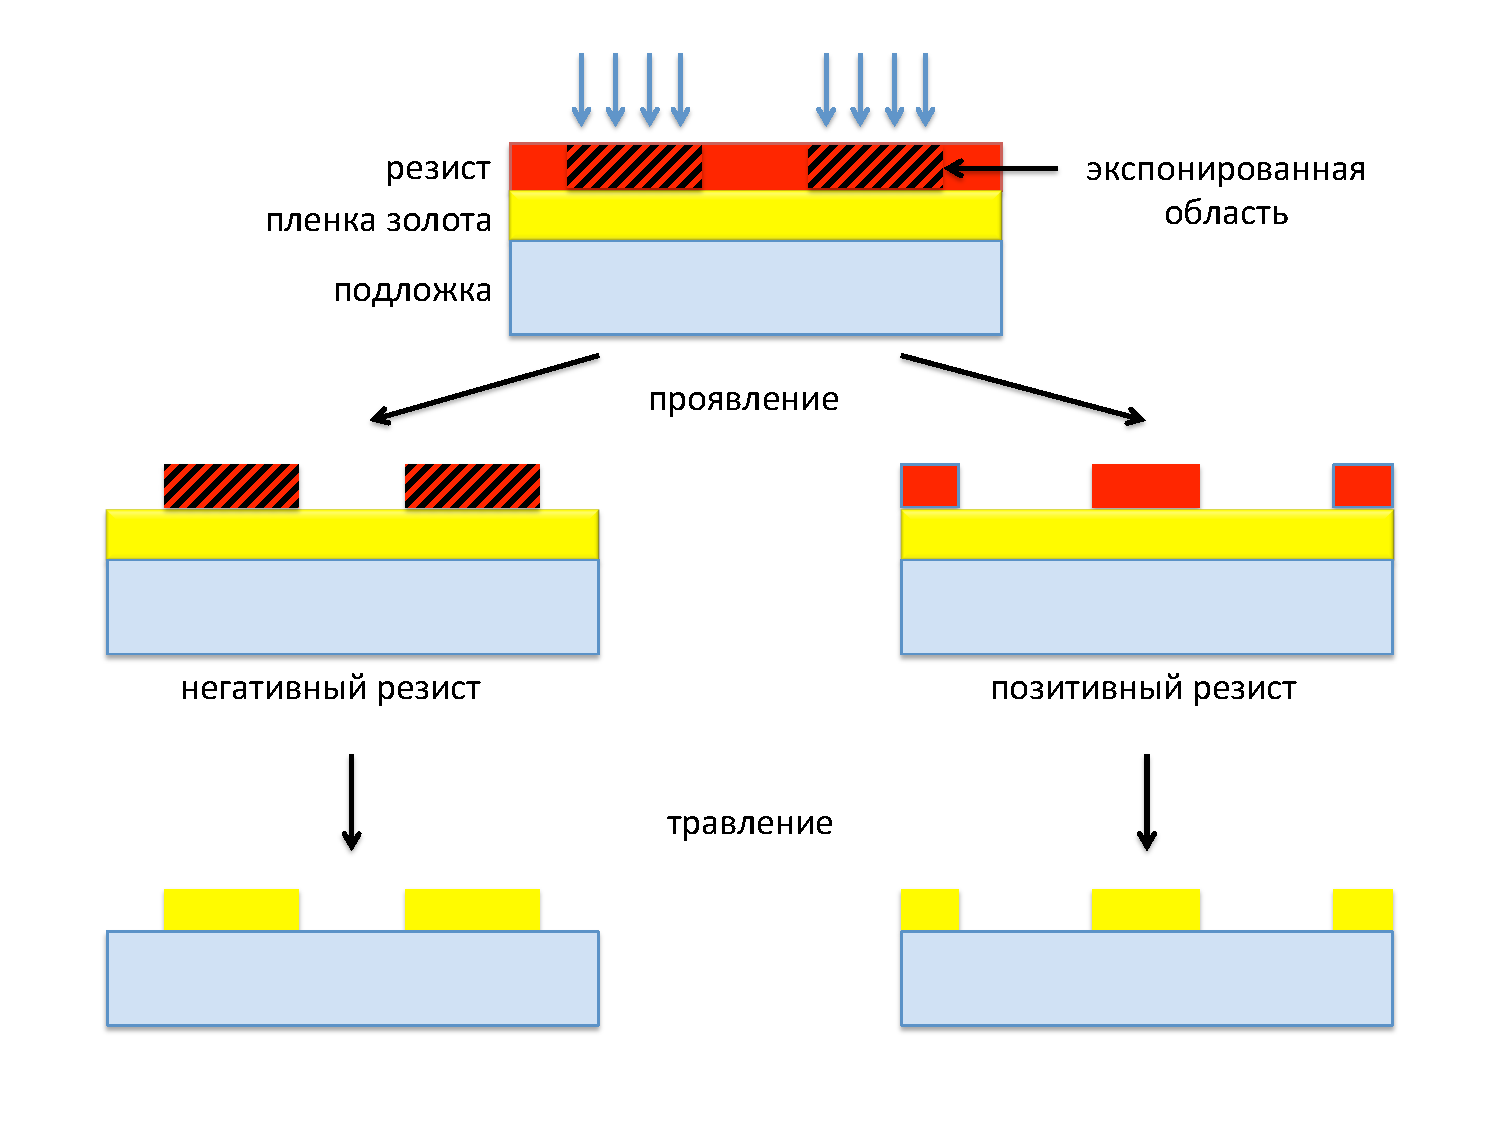
\includegraphics[width=12cm]{img/litography.pdf}}
\caption{Основные этапы литографического процесса с использованием негативного (слева) и позитивного (справа) резистов.}
\label{img:litography}
\end{figure}

Создание структур субмикронных размеров возможно с помощью электронно-лучевой литографии (ЭЛЛ) \cite{SPIEnanofabrication}, позволяющий получать объекты с характерным размером меньше 1 нм. Существуют две системы ЭЛЛ --- сканирующая и проекционная. При использовании сканирующей системы резист экспонируется фокусированным потоком электронов. В сканирующей ЭЛЛ электронный луч перемещается в плоскости рисунка и производит его последовательное экспонирование. Информация для управления электронным лучом хранится в памяти управляющего компьютера, поэтому не нужно применять какие-либо шаблоны. Однако последовательное сканирование всего рисунка приводит к значительному увеличению времени экспонирования. В проекционной системе широкий несфокусированный поток электронов можно использовать для получения всего рисунка в течение одной экспозиции. Соответствующая электронная проекционная система описана в \cite{projectelectron}. В этой системе фотокатод расположен на поверхности оптической маски с заданным рисунком. Ультрафиолетовые лучи облучают фотокатодный слой через маску, что вызывает эмиссию электронов с фотокатода в облученных местах рисунка. Эти электроны проецируются на поверхность резиста с помощью однородных электростатических и магнитных полей. В результате на всей площади подложки рисунок создается за одну экспозицию. На рис.\ref{img:EBLscheme} представлены схемы установок для сканирующей (слева) и проекционной (справа) систем ЭЛЛ. 

\begin{figure}
\center{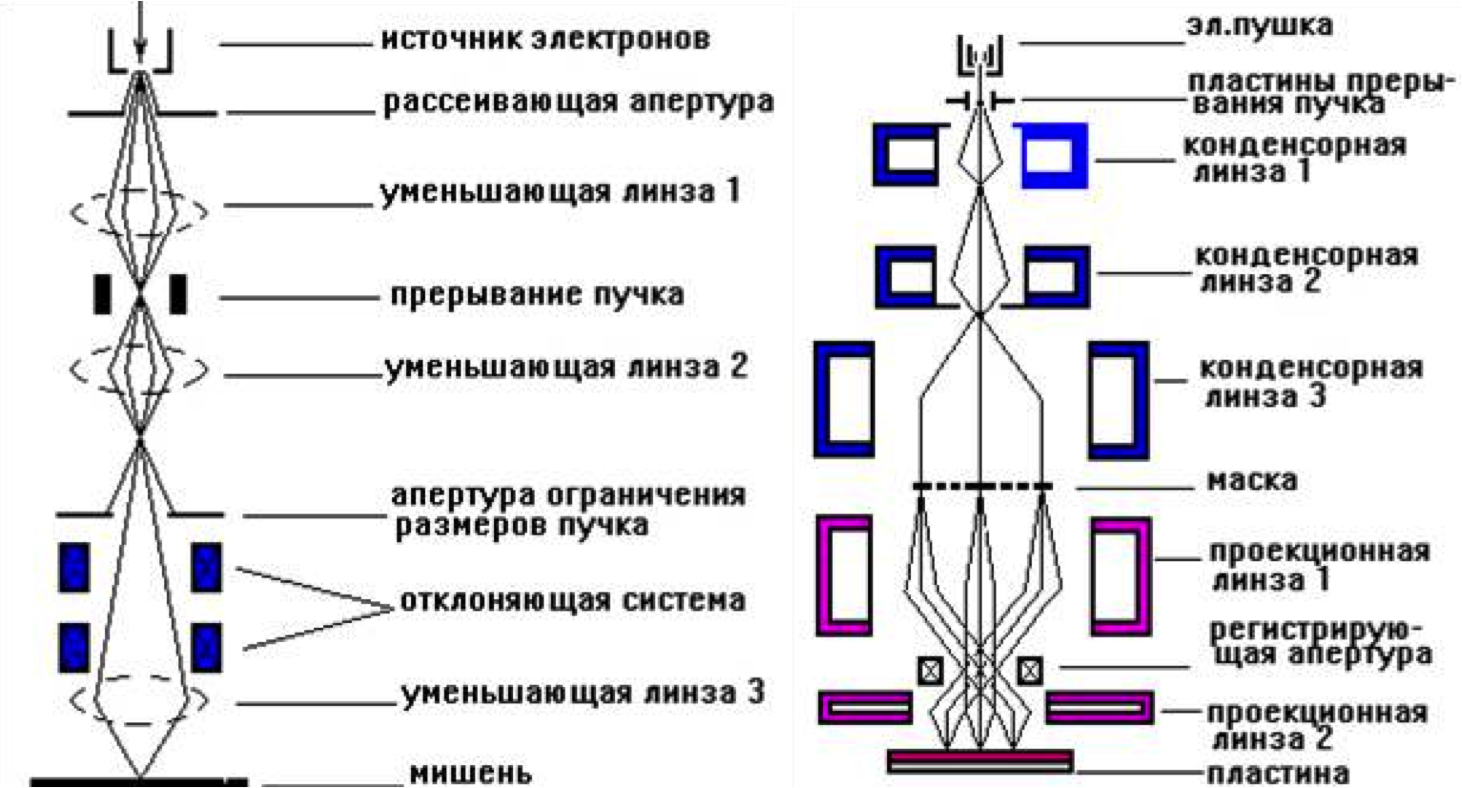
\includegraphics[width=15cm]{img/EBLschemes.png}}
\caption{Схемы установок для сканирующей (слева) и проекционной (справа) систем ЭЛЛ\cite{nanotechnologybook}.}
\label{img:EBLscheme}
\end{figure}

